% Options for packages loaded elsewhere
\PassOptionsToPackage{unicode}{hyperref}
\PassOptionsToPackage{hyphens}{url}
\PassOptionsToPackage{dvipsnames,svgnames,x11names}{xcolor}
%
\documentclass[
  letterpaper,
  DIV=11,
  numbers=noendperiod]{scrartcl}

\usepackage{amsmath,amssymb}
\usepackage{iftex}
\ifPDFTeX
  \usepackage[T1]{fontenc}
  \usepackage[utf8]{inputenc}
  \usepackage{textcomp} % provide euro and other symbols
\else % if luatex or xetex
  \usepackage{unicode-math}
  \defaultfontfeatures{Scale=MatchLowercase}
  \defaultfontfeatures[\rmfamily]{Ligatures=TeX,Scale=1}
\fi
\usepackage{lmodern}
\ifPDFTeX\else  
    % xetex/luatex font selection
\fi
% Use upquote if available, for straight quotes in verbatim environments
\IfFileExists{upquote.sty}{\usepackage{upquote}}{}
\IfFileExists{microtype.sty}{% use microtype if available
  \usepackage[]{microtype}
  \UseMicrotypeSet[protrusion]{basicmath} % disable protrusion for tt fonts
}{}
\makeatletter
\@ifundefined{KOMAClassName}{% if non-KOMA class
  \IfFileExists{parskip.sty}{%
    \usepackage{parskip}
  }{% else
    \setlength{\parindent}{0pt}
    \setlength{\parskip}{6pt plus 2pt minus 1pt}}
}{% if KOMA class
  \KOMAoptions{parskip=half}}
\makeatother
\usepackage{xcolor}
\setlength{\emergencystretch}{3em} % prevent overfull lines
\setcounter{secnumdepth}{-\maxdimen} % remove section numbering
% Make \paragraph and \subparagraph free-standing
\ifx\paragraph\undefined\else
  \let\oldparagraph\paragraph
  \renewcommand{\paragraph}[1]{\oldparagraph{#1}\mbox{}}
\fi
\ifx\subparagraph\undefined\else
  \let\oldsubparagraph\subparagraph
  \renewcommand{\subparagraph}[1]{\oldsubparagraph{#1}\mbox{}}
\fi

\usepackage{color}
\usepackage{fancyvrb}
\newcommand{\VerbBar}{|}
\newcommand{\VERB}{\Verb[commandchars=\\\{\}]}
\DefineVerbatimEnvironment{Highlighting}{Verbatim}{commandchars=\\\{\}}
% Add ',fontsize=\small' for more characters per line
\usepackage{framed}
\definecolor{shadecolor}{RGB}{241,243,245}
\newenvironment{Shaded}{\begin{snugshade}}{\end{snugshade}}
\newcommand{\AlertTok}[1]{\textcolor[rgb]{0.68,0.00,0.00}{#1}}
\newcommand{\AnnotationTok}[1]{\textcolor[rgb]{0.37,0.37,0.37}{#1}}
\newcommand{\AttributeTok}[1]{\textcolor[rgb]{0.40,0.45,0.13}{#1}}
\newcommand{\BaseNTok}[1]{\textcolor[rgb]{0.68,0.00,0.00}{#1}}
\newcommand{\BuiltInTok}[1]{\textcolor[rgb]{0.00,0.23,0.31}{#1}}
\newcommand{\CharTok}[1]{\textcolor[rgb]{0.13,0.47,0.30}{#1}}
\newcommand{\CommentTok}[1]{\textcolor[rgb]{0.37,0.37,0.37}{#1}}
\newcommand{\CommentVarTok}[1]{\textcolor[rgb]{0.37,0.37,0.37}{\textit{#1}}}
\newcommand{\ConstantTok}[1]{\textcolor[rgb]{0.56,0.35,0.01}{#1}}
\newcommand{\ControlFlowTok}[1]{\textcolor[rgb]{0.00,0.23,0.31}{#1}}
\newcommand{\DataTypeTok}[1]{\textcolor[rgb]{0.68,0.00,0.00}{#1}}
\newcommand{\DecValTok}[1]{\textcolor[rgb]{0.68,0.00,0.00}{#1}}
\newcommand{\DocumentationTok}[1]{\textcolor[rgb]{0.37,0.37,0.37}{\textit{#1}}}
\newcommand{\ErrorTok}[1]{\textcolor[rgb]{0.68,0.00,0.00}{#1}}
\newcommand{\ExtensionTok}[1]{\textcolor[rgb]{0.00,0.23,0.31}{#1}}
\newcommand{\FloatTok}[1]{\textcolor[rgb]{0.68,0.00,0.00}{#1}}
\newcommand{\FunctionTok}[1]{\textcolor[rgb]{0.28,0.35,0.67}{#1}}
\newcommand{\ImportTok}[1]{\textcolor[rgb]{0.00,0.46,0.62}{#1}}
\newcommand{\InformationTok}[1]{\textcolor[rgb]{0.37,0.37,0.37}{#1}}
\newcommand{\KeywordTok}[1]{\textcolor[rgb]{0.00,0.23,0.31}{#1}}
\newcommand{\NormalTok}[1]{\textcolor[rgb]{0.00,0.23,0.31}{#1}}
\newcommand{\OperatorTok}[1]{\textcolor[rgb]{0.37,0.37,0.37}{#1}}
\newcommand{\OtherTok}[1]{\textcolor[rgb]{0.00,0.23,0.31}{#1}}
\newcommand{\PreprocessorTok}[1]{\textcolor[rgb]{0.68,0.00,0.00}{#1}}
\newcommand{\RegionMarkerTok}[1]{\textcolor[rgb]{0.00,0.23,0.31}{#1}}
\newcommand{\SpecialCharTok}[1]{\textcolor[rgb]{0.37,0.37,0.37}{#1}}
\newcommand{\SpecialStringTok}[1]{\textcolor[rgb]{0.13,0.47,0.30}{#1}}
\newcommand{\StringTok}[1]{\textcolor[rgb]{0.13,0.47,0.30}{#1}}
\newcommand{\VariableTok}[1]{\textcolor[rgb]{0.07,0.07,0.07}{#1}}
\newcommand{\VerbatimStringTok}[1]{\textcolor[rgb]{0.13,0.47,0.30}{#1}}
\newcommand{\WarningTok}[1]{\textcolor[rgb]{0.37,0.37,0.37}{\textit{#1}}}

\providecommand{\tightlist}{%
  \setlength{\itemsep}{0pt}\setlength{\parskip}{0pt}}\usepackage{longtable,booktabs,array}
\usepackage{calc} % for calculating minipage widths
% Correct order of tables after \paragraph or \subparagraph
\usepackage{etoolbox}
\makeatletter
\patchcmd\longtable{\par}{\if@noskipsec\mbox{}\fi\par}{}{}
\makeatother
% Allow footnotes in longtable head/foot
\IfFileExists{footnotehyper.sty}{\usepackage{footnotehyper}}{\usepackage{footnote}}
\makesavenoteenv{longtable}
\usepackage{graphicx}
\makeatletter
\def\maxwidth{\ifdim\Gin@nat@width>\linewidth\linewidth\else\Gin@nat@width\fi}
\def\maxheight{\ifdim\Gin@nat@height>\textheight\textheight\else\Gin@nat@height\fi}
\makeatother
% Scale images if necessary, so that they will not overflow the page
% margins by default, and it is still possible to overwrite the defaults
% using explicit options in \includegraphics[width, height, ...]{}
\setkeys{Gin}{width=\maxwidth,height=\maxheight,keepaspectratio}
% Set default figure placement to htbp
\makeatletter
\def\fps@figure{htbp}
\makeatother

\KOMAoption{captions}{tableheading}
\makeatletter
\makeatother
\makeatletter
\makeatother
\makeatletter
\@ifpackageloaded{caption}{}{\usepackage{caption}}
\AtBeginDocument{%
\ifdefined\contentsname
  \renewcommand*\contentsname{Table of contents}
\else
  \newcommand\contentsname{Table of contents}
\fi
\ifdefined\listfigurename
  \renewcommand*\listfigurename{List of Figures}
\else
  \newcommand\listfigurename{List of Figures}
\fi
\ifdefined\listtablename
  \renewcommand*\listtablename{List of Tables}
\else
  \newcommand\listtablename{List of Tables}
\fi
\ifdefined\figurename
  \renewcommand*\figurename{Figure}
\else
  \newcommand\figurename{Figure}
\fi
\ifdefined\tablename
  \renewcommand*\tablename{Table}
\else
  \newcommand\tablename{Table}
\fi
}
\@ifpackageloaded{float}{}{\usepackage{float}}
\floatstyle{ruled}
\@ifundefined{c@chapter}{\newfloat{codelisting}{h}{lop}}{\newfloat{codelisting}{h}{lop}[chapter]}
\floatname{codelisting}{Listing}
\newcommand*\listoflistings{\listof{codelisting}{List of Listings}}
\makeatother
\makeatletter
\@ifpackageloaded{caption}{}{\usepackage{caption}}
\@ifpackageloaded{subcaption}{}{\usepackage{subcaption}}
\makeatother
\makeatletter
\@ifpackageloaded{tcolorbox}{}{\usepackage[skins,breakable]{tcolorbox}}
\makeatother
\makeatletter
\@ifundefined{shadecolor}{\definecolor{shadecolor}{rgb}{.97, .97, .97}}
\makeatother
\makeatletter
\makeatother
\makeatletter
\makeatother
\ifLuaTeX
  \usepackage{selnolig}  % disable illegal ligatures
\fi
\IfFileExists{bookmark.sty}{\usepackage{bookmark}}{\usepackage{hyperref}}
\IfFileExists{xurl.sty}{\usepackage{xurl}}{} % add URL line breaks if available
\urlstyle{same} % disable monospaced font for URLs
\hypersetup{
  pdftitle={Class 07: Clustering and PCA},
  pdfauthor={Alex Cagle},
  colorlinks=true,
  linkcolor={blue},
  filecolor={Maroon},
  citecolor={Blue},
  urlcolor={Blue},
  pdfcreator={LaTeX via pandoc}}

\title{Class 07: Clustering and PCA}
\author{Alex Cagle}
\date{}

\begin{document}
\maketitle
\ifdefined\Shaded\renewenvironment{Shaded}{\begin{tcolorbox}[interior hidden, borderline west={3pt}{0pt}{shadecolor}, enhanced, sharp corners, boxrule=0pt, frame hidden, breakable]}{\end{tcolorbox}}\fi

\hypertarget{clustering}{%
\subsection{Clustering}\label{clustering}}

We can use the \texttt{rnorm()} function to get random numbers from a
normal distribution around a given \texttt{mean}.

\begin{Shaded}
\begin{Highlighting}[]
\FunctionTok{hist}\NormalTok{(}\FunctionTok{rnorm}\NormalTok{(}\DecValTok{5000}\NormalTok{, }\AttributeTok{mean=}\DecValTok{1}\NormalTok{))}
\end{Highlighting}
\end{Shaded}

\begin{figure}[H]

{\centering 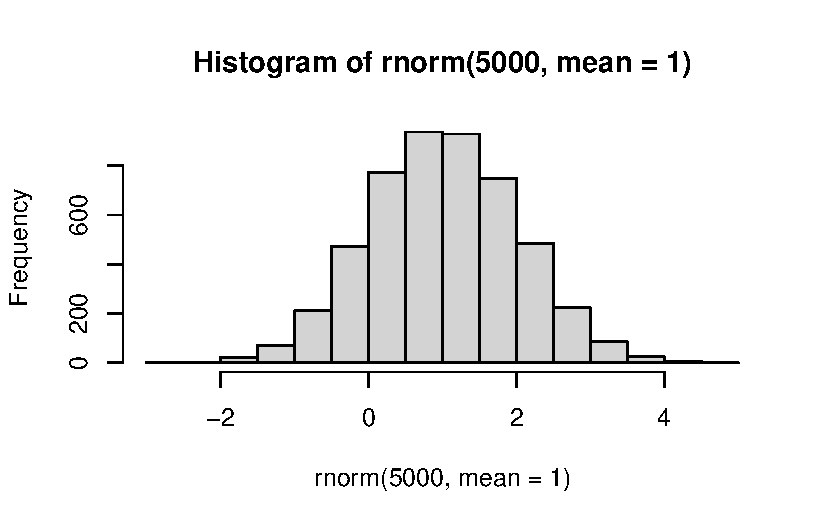
\includegraphics{Lab-7_files/figure-pdf/unnamed-chunk-1-1.pdf}

}

\end{figure}

Let's get 30 points with a mean of 3.

\begin{Shaded}
\begin{Highlighting}[]
\NormalTok{rnorm1 }\OtherTok{\textless{}{-}} \FunctionTok{rnorm}\NormalTok{(}\DecValTok{30}\NormalTok{, }\AttributeTok{mean=}\DecValTok{3}\NormalTok{)}
\NormalTok{rnorm1}
\end{Highlighting}
\end{Shaded}

\begin{verbatim}
 [1] 2.685636 1.856482 1.652886 2.118168 2.637088 3.360176 1.187066 3.285751
 [9] 4.144507 3.897459 2.737182 1.959894 3.174756 2.126037 2.484987 4.327654
[17] 3.870147 2.872417 2.936440 2.472300 1.987376 1.911272 2.096007 2.821700
[25] 1.689848 3.561290 3.760353 4.296043 3.668240 3.041588
\end{verbatim}

\begin{Shaded}
\begin{Highlighting}[]
\CommentTok{\# rnorm2 \textless{}{-} rnorm(30, mean={-}30)}
\CommentTok{\# rnorm2}

\CommentTok{\# x \textless{}{-} c(rnorm1, rnorm2)}
\CommentTok{\# x}

\CommentTok{\# cbind(rnorm1, rnorm2)}

\CommentTok{\# rev( c(1:5) )}

\CommentTok{\# y \textless{}{-} cbind( rev(rnorm1), rev(rnorm2) )}
\CommentTok{\# y}
\end{Highlighting}
\end{Shaded}

\begin{Shaded}
\begin{Highlighting}[]
\NormalTok{tmp }\OtherTok{\textless{}{-}} \FunctionTok{c}\NormalTok{(}\FunctionTok{rnorm}\NormalTok{(}\DecValTok{30}\NormalTok{, }\AttributeTok{mean=}\DecValTok{3}\NormalTok{), }\FunctionTok{rnorm}\NormalTok{(}\DecValTok{30}\NormalTok{, }\AttributeTok{mean=}\SpecialCharTok{{-}}\DecValTok{3}\NormalTok{))}
\NormalTok{tmp}
\end{Highlighting}
\end{Shaded}

\begin{verbatim}
 [1]  3.9993083  4.8156385  1.8638811  2.9563276  4.1117662  3.7916146
 [7]  3.5704448  0.6464429  2.4453977  4.8446939  2.1598117  1.3365666
[13]  2.6124229  2.6177808  0.7039838  3.3837175  2.2726193  3.6167278
[19]  3.7680698  2.6425843  2.9512371  2.5609873  3.6531720  3.9635759
[25]  4.0135697  2.0394009  2.4552453  4.4565114  2.4306618  3.0055968
[31] -3.1802843 -2.1161673 -2.1651039 -2.3890947 -2.5233007 -3.7087414
[37] -2.7425496 -2.5899740 -2.4219931 -2.3903431 -5.5333943 -2.5935633
[43] -2.5072866 -1.6542928 -2.1850577 -2.7193581 -2.0589103 -2.8393720
[49] -1.5616040 -4.4532644 -1.7159841 -3.2306124 -1.9276014 -2.6505754
[55] -3.4167590 -2.8544513 -2.9596110 -2.1137610 -2.0002680 -3.0132642
\end{verbatim}

\begin{Shaded}
\begin{Highlighting}[]
\CommentTok{\# Put these two together}
\NormalTok{x }\OtherTok{\textless{}{-}} \FunctionTok{cbind}\NormalTok{(}\AttributeTok{x=}\NormalTok{tmp, }\AttributeTok{y=}\FunctionTok{rev}\NormalTok{(tmp))}
\NormalTok{x}
\end{Highlighting}
\end{Shaded}

\begin{verbatim}
               x          y
 [1,]  3.9993083 -3.0132642
 [2,]  4.8156385 -2.0002680
 [3,]  1.8638811 -2.1137610
 [4,]  2.9563276 -2.9596110
 [5,]  4.1117662 -2.8544513
 [6,]  3.7916146 -3.4167590
 [7,]  3.5704448 -2.6505754
 [8,]  0.6464429 -1.9276014
 [9,]  2.4453977 -3.2306124
[10,]  4.8446939 -1.7159841
[11,]  2.1598117 -4.4532644
[12,]  1.3365666 -1.5616040
[13,]  2.6124229 -2.8393720
[14,]  2.6177808 -2.0589103
[15,]  0.7039838 -2.7193581
[16,]  3.3837175 -2.1850577
[17,]  2.2726193 -1.6542928
[18,]  3.6167278 -2.5072866
[19,]  3.7680698 -2.5935633
[20,]  2.6425843 -5.5333943
[21,]  2.9512371 -2.3903431
[22,]  2.5609873 -2.4219931
[23,]  3.6531720 -2.5899740
[24,]  3.9635759 -2.7425496
[25,]  4.0135697 -3.7087414
[26,]  2.0394009 -2.5233007
[27,]  2.4552453 -2.3890947
[28,]  4.4565114 -2.1651039
[29,]  2.4306618 -2.1161673
[30,]  3.0055968 -3.1802843
[31,] -3.1802843  3.0055968
[32,] -2.1161673  2.4306618
[33,] -2.1651039  4.4565114
[34,] -2.3890947  2.4552453
[35,] -2.5233007  2.0394009
[36,] -3.7087414  4.0135697
[37,] -2.7425496  3.9635759
[38,] -2.5899740  3.6531720
[39,] -2.4219931  2.5609873
[40,] -2.3903431  2.9512371
[41,] -5.5333943  2.6425843
[42,] -2.5935633  3.7680698
[43,] -2.5072866  3.6167278
[44,] -1.6542928  2.2726193
[45,] -2.1850577  3.3837175
[46,] -2.7193581  0.7039838
[47,] -2.0589103  2.6177808
[48,] -2.8393720  2.6124229
[49,] -1.5616040  1.3365666
[50,] -4.4532644  2.1598117
[51,] -1.7159841  4.8446939
[52,] -3.2306124  2.4453977
[53,] -1.9276014  0.6464429
[54,] -2.6505754  3.5704448
[55,] -3.4167590  3.7916146
[56,] -2.8544513  4.1117662
[57,] -2.9596110  2.9563276
[58,] -2.1137610  1.8638811
[59,] -2.0002680  4.8156385
[60,] -3.0132642  3.9993083
\end{verbatim}

\begin{Shaded}
\begin{Highlighting}[]
\FunctionTok{plot}\NormalTok{(x)}
\end{Highlighting}
\end{Shaded}

\begin{figure}[H]

{\centering 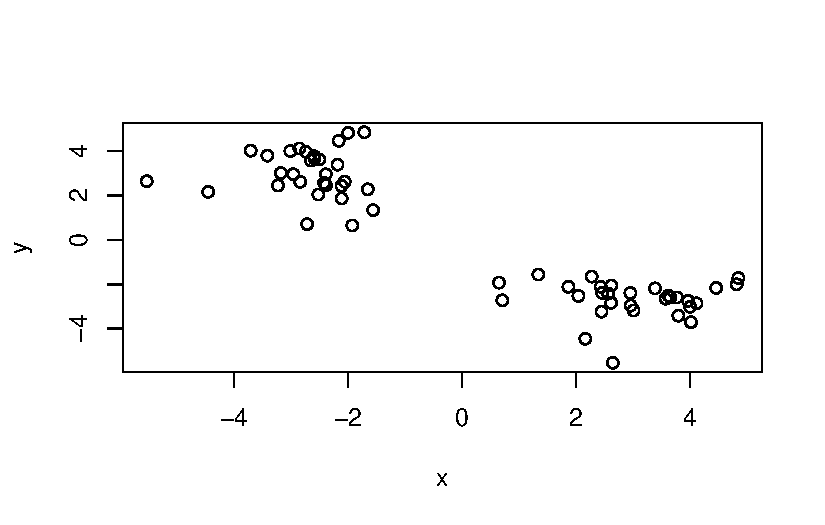
\includegraphics{Lab-7_files/figure-pdf/unnamed-chunk-4-1.pdf}

}

\end{figure}

\hypertarget{k-means-clustering}{%
\subsection{K-means clustering}\label{k-means-clustering}}

Very popular clustering method for big data sets.

\begin{Shaded}
\begin{Highlighting}[]
\NormalTok{km }\OtherTok{\textless{}{-}} \FunctionTok{kmeans}\NormalTok{(x, }\DecValTok{2}\NormalTok{)}
\NormalTok{km}
\end{Highlighting}
\end{Shaded}

\begin{verbatim}
K-means clustering with 2 clusters of sizes 30, 30

Cluster means:
          x         y
1  2.989659 -2.673885
2 -2.673885  2.989659

Clustering vector:
 [1] 1 1 1 1 1 1 1 1 1 1 1 1 1 1 1 1 1 1 1 1 1 1 1 1 1 1 1 1 1 1 2 2 2 2 2 2 2 2
[39] 2 2 2 2 2 2 2 2 2 2 2 2 2 2 2 2 2 2 2 2 2 2

Within cluster sum of squares by cluster:
[1] 53.87133 53.87133
 (between_SS / total_SS =  89.9 %)

Available components:

[1] "cluster"      "centers"      "totss"        "withinss"     "tot.withinss"
[6] "betweenss"    "size"         "iter"         "ifault"      
\end{verbatim}

\begin{Shaded}
\begin{Highlighting}[]
\NormalTok{km}\SpecialCharTok{$}\NormalTok{cluster}
\end{Highlighting}
\end{Shaded}

\begin{verbatim}
 [1] 1 1 1 1 1 1 1 1 1 1 1 1 1 1 1 1 1 1 1 1 1 1 1 1 1 1 1 1 1 1 2 2 2 2 2 2 2 2
[39] 2 2 2 2 2 2 2 2 2 2 2 2 2 2 2 2 2 2 2 2 2 2
\end{verbatim}

\begin{Shaded}
\begin{Highlighting}[]
\NormalTok{km}\SpecialCharTok{$}\NormalTok{size}
\end{Highlighting}
\end{Shaded}

\begin{verbatim}
[1] 30 30
\end{verbatim}

\begin{Shaded}
\begin{Highlighting}[]
\NormalTok{km}\SpecialCharTok{$}\NormalTok{centers}
\end{Highlighting}
\end{Shaded}

\begin{verbatim}
          x         y
1  2.989659 -2.673885
2 -2.673885  2.989659
\end{verbatim}

\begin{quote}
Q: How many points are in each cluster?
\end{quote}

\begin{Shaded}
\begin{Highlighting}[]
\CommentTok{\# We can use km$size to see how many points are in each cluster}
\CommentTok{\# In this case, there are 30 points in each cluster}
\NormalTok{km}\SpecialCharTok{$}\NormalTok{size}
\end{Highlighting}
\end{Shaded}

\begin{verbatim}
[1] 30 30
\end{verbatim}

\begin{quote}
Q: What `component' of your result object details:

\begin{itemize}
\item
  cluster size?
\item
  cluster assignment/membership?
\item
  cluster center?
\end{itemize}
\end{quote}

\begin{Shaded}
\begin{Highlighting}[]
\CommentTok{\# Cluster size}
\NormalTok{km}\SpecialCharTok{$}\NormalTok{size}
\end{Highlighting}
\end{Shaded}

\begin{verbatim}
[1] 30 30
\end{verbatim}

\begin{Shaded}
\begin{Highlighting}[]
\CommentTok{\# Membership}
\NormalTok{km}\SpecialCharTok{$}\NormalTok{cluster}
\end{Highlighting}
\end{Shaded}

\begin{verbatim}
 [1] 1 1 1 1 1 1 1 1 1 1 1 1 1 1 1 1 1 1 1 1 1 1 1 1 1 1 1 1 1 1 2 2 2 2 2 2 2 2
[39] 2 2 2 2 2 2 2 2 2 2 2 2 2 2 2 2 2 2 2 2 2 2
\end{verbatim}

\begin{Shaded}
\begin{Highlighting}[]
\CommentTok{\# Cluster center}
\NormalTok{km}\SpecialCharTok{$}\NormalTok{centers}
\end{Highlighting}
\end{Shaded}

\begin{verbatim}
          x         y
1  2.989659 -2.673885
2 -2.673885  2.989659
\end{verbatim}

\begin{quote}
Q: Plot x colored by the kmeans cluster assignment and add cluster
centers as blue points.
\end{quote}

\begin{Shaded}
\begin{Highlighting}[]
\NormalTok{mycols }\OtherTok{\textless{}{-}}\NormalTok{ km}\SpecialCharTok{$}\NormalTok{cluster}
\NormalTok{mycols }\OtherTok{\textless{}{-}}\NormalTok{ mycols }\SpecialCharTok{+} \DecValTok{1}
\FunctionTok{plot}\NormalTok{(x, }\AttributeTok{col =}\NormalTok{ mycols)}
\FunctionTok{points}\NormalTok{(km}\SpecialCharTok{$}\NormalTok{centers, }\AttributeTok{col =} \StringTok{\textquotesingle{}blue\textquotesingle{}}\NormalTok{, }\AttributeTok{pch =} \DecValTok{15}\NormalTok{, }\AttributeTok{cex =} \DecValTok{3}\NormalTok{)}
\end{Highlighting}
\end{Shaded}

\begin{figure}[H]

{\centering 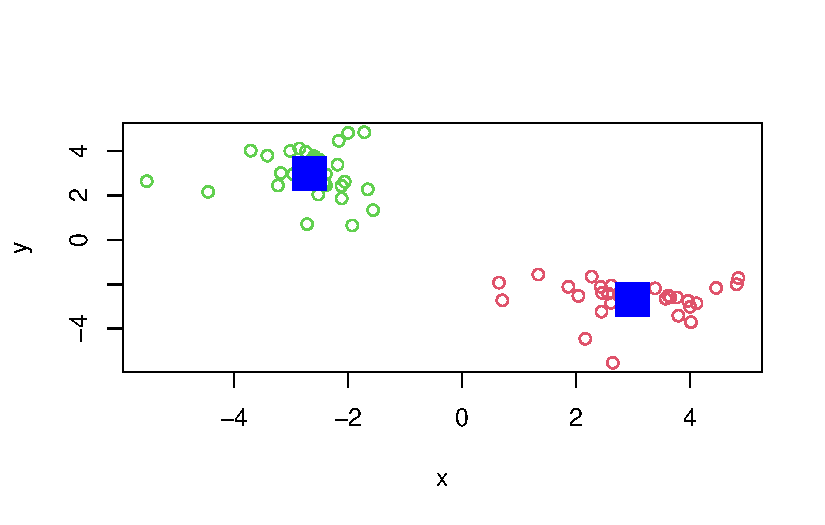
\includegraphics{Lab-7_files/figure-pdf/unnamed-chunk-9-1.pdf}

}

\end{figure}

\begin{quote}
Q: Let's cluster into 3 groups or same `x' data and make a plot.
\end{quote}

\begin{Shaded}
\begin{Highlighting}[]
\NormalTok{km2 }\OtherTok{\textless{}{-}} \FunctionTok{kmeans}\NormalTok{(x, }\DecValTok{3}\NormalTok{)}
\NormalTok{km2}
\end{Highlighting}
\end{Shaded}

\begin{verbatim}
K-means clustering with 3 clusters of sizes 16, 14, 30

Cluster means:
          x         y
1  3.787082 -2.863554
2  2.078317 -2.457120
3 -2.673885  2.989659

Clustering vector:
 [1] 1 1 2 1 1 1 1 2 2 1 2 2 2 2 2 1 2 1 1 1 2 2 1 1 1 2 2 1 2 1 3 3 3 3 3 3 3 3
[39] 3 3 3 3 3 3 3 3 3 3 3 3 3 3 3 3 3 3 3 3 3 3

Within cluster sum of squares by cluster:
[1] 17.35073 13.48542 53.87133
 (between_SS / total_SS =  92.1 %)

Available components:

[1] "cluster"      "centers"      "totss"        "withinss"     "tot.withinss"
[6] "betweenss"    "size"         "iter"         "ifault"      
\end{verbatim}

\begin{Shaded}
\begin{Highlighting}[]
\FunctionTok{plot}\NormalTok{(x, }\AttributeTok{col =}\NormalTok{ km2}\SpecialCharTok{$}\NormalTok{cluster)}
\FunctionTok{points}\NormalTok{(km2}\SpecialCharTok{$}\NormalTok{centers, }\AttributeTok{col =} \StringTok{\textquotesingle{}blue\textquotesingle{}}\NormalTok{, }\AttributeTok{pch =} \DecValTok{15}\NormalTok{, }\AttributeTok{cex =} \DecValTok{3}\NormalTok{)}
\end{Highlighting}
\end{Shaded}

\begin{figure}[H]

{\centering 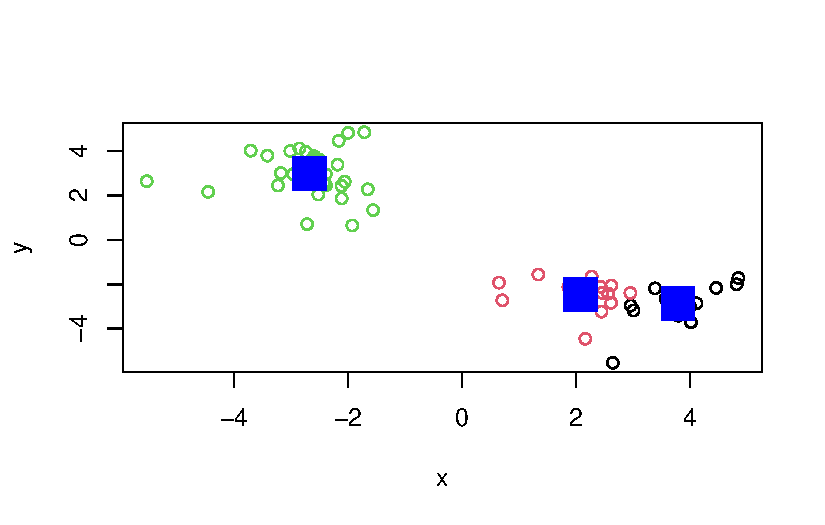
\includegraphics{Lab-7_files/figure-pdf/unnamed-chunk-10-1.pdf}

}

\end{figure}

\hypertarget{hierarchical-clustering}{%
\section{Hierarchical Clustering}\label{hierarchical-clustering}}

We can use the \texttt{hclust()} function for hierarchical clustering.
Unlike \texttt{kmeans()} where we could just pass in our own data as
input, we need to give \texttt{hclust()} a ``distance matrix'' (how far
apart the points are, e.g.~Euclidean distance \texttt{dist()} or other
types of distance).

We will use the \texttt{dist()} function to start with.

\begin{Shaded}
\begin{Highlighting}[]
\NormalTok{d }\OtherTok{\textless{}{-}} \FunctionTok{dist}\NormalTok{(x)}
\NormalTok{hc }\OtherTok{\textless{}{-}} \FunctionTok{hclust}\NormalTok{(d)}
\NormalTok{hc}
\end{Highlighting}
\end{Shaded}

\begin{verbatim}

Call:
hclust(d = d)

Cluster method   : complete 
Distance         : euclidean 
Number of objects: 60 
\end{verbatim}

\begin{Shaded}
\begin{Highlighting}[]
\FunctionTok{plot}\NormalTok{(hc)}
\end{Highlighting}
\end{Shaded}

\begin{figure}[H]

{\centering 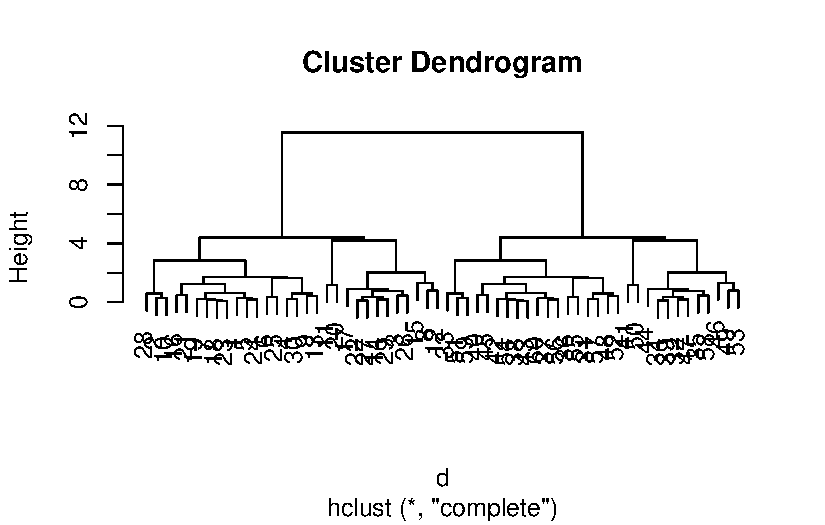
\includegraphics{Lab-7_files/figure-pdf/unnamed-chunk-12-1.pdf}

}

\end{figure}

I can now ``cut'' my tree with the \texttt{cutree()} function to yield a
cluster membership vector.

\begin{Shaded}
\begin{Highlighting}[]
\NormalTok{grps }\OtherTok{\textless{}{-}} \FunctionTok{cutree}\NormalTok{(hc, }\AttributeTok{h=}\DecValTok{8}\NormalTok{)}
\NormalTok{grps}
\end{Highlighting}
\end{Shaded}

\begin{verbatim}
 [1] 1 1 1 1 1 1 1 1 1 1 1 1 1 1 1 1 1 1 1 1 1 1 1 1 1 1 1 1 1 1 2 2 2 2 2 2 2 2
[39] 2 2 2 2 2 2 2 2 2 2 2 2 2 2 2 2 2 2 2 2 2 2
\end{verbatim}

\begin{Shaded}
\begin{Highlighting}[]
\FunctionTok{plot}\NormalTok{(x, }\AttributeTok{col =}\NormalTok{ grps)}
\end{Highlighting}
\end{Shaded}

\begin{figure}[H]

{\centering 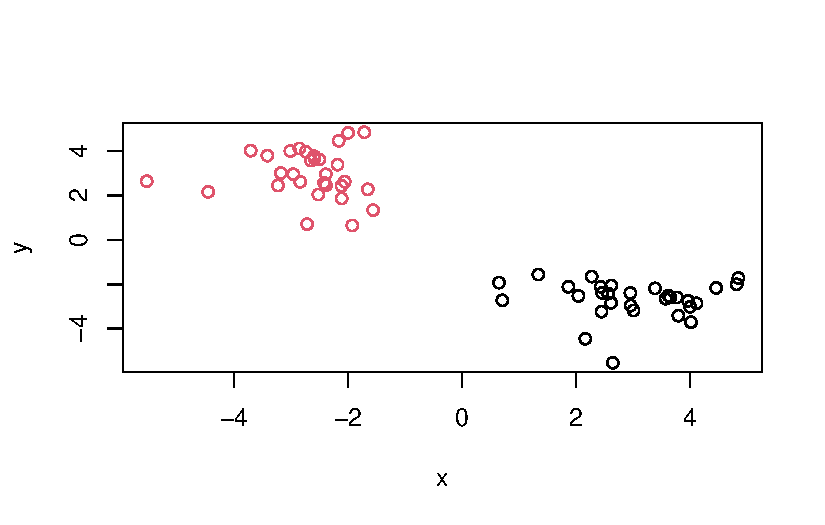
\includegraphics{Lab-7_files/figure-pdf/unnamed-chunk-14-1.pdf}

}

\end{figure}

You can also tell \texttt{cutree()} to cut where it yields ``k'' groups.

\begin{Shaded}
\begin{Highlighting}[]
\FunctionTok{cutree}\NormalTok{(hc, }\AttributeTok{k=}\DecValTok{2}\NormalTok{)}
\end{Highlighting}
\end{Shaded}

\begin{verbatim}
 [1] 1 1 1 1 1 1 1 1 1 1 1 1 1 1 1 1 1 1 1 1 1 1 1 1 1 1 1 1 1 1 2 2 2 2 2 2 2 2
[39] 2 2 2 2 2 2 2 2 2 2 2 2 2 2 2 2 2 2 2 2 2 2
\end{verbatim}

\hypertarget{lab-7-principal-component-analysis-pca}{%
\section{Lab 7: Principal Component Analysis
(PCA)}\label{lab-7-principal-component-analysis-pca}}

\hypertarget{pca-of-uk-foods}{%
\subsection{PCA of UK Foods}\label{pca-of-uk-foods}}

\begin{Shaded}
\begin{Highlighting}[]
\NormalTok{url }\OtherTok{\textless{}{-}} \StringTok{"https://tinyurl.com/UK{-}foods"}
\NormalTok{x }\OtherTok{\textless{}{-}} \FunctionTok{read.csv}\NormalTok{(url, }\AttributeTok{row.names =} \DecValTok{1}\NormalTok{)}

\CommentTok{\# Q2: This solves the \textquotesingle{}row{-}names problem\textquotesingle{}. In my opinion, this way is better since it automatically sets the first column as the names column, which makes operating on the dataset easier.}
\end{Highlighting}
\end{Shaded}

\begin{Shaded}
\begin{Highlighting}[]
\CommentTok{\# Finding number of rows and columns}
\FunctionTok{dim}\NormalTok{(x)}
\end{Highlighting}
\end{Shaded}

\begin{verbatim}
[1] 17  4
\end{verbatim}

\begin{Shaded}
\begin{Highlighting}[]
\CommentTok{\# Q1: We have 17 rows and 4 columns, where each column is a country.}
\end{Highlighting}
\end{Shaded}

\begin{Shaded}
\begin{Highlighting}[]
\CommentTok{\# Using head to preview first 6 rows}
\FunctionTok{head}\NormalTok{(x)}
\end{Highlighting}
\end{Shaded}

\begin{verbatim}
               England Wales Scotland N.Ireland
Cheese             105   103      103        66
Carcass_meat       245   227      242       267
Other_meat         685   803      750       586
Fish               147   160      122        93
Fats_and_oils      193   235      184       209
Sugars             156   175      147       139
\end{verbatim}

\begin{Shaded}
\begin{Highlighting}[]
\CommentTok{\# Generating barplot}
\FunctionTok{barplot}\NormalTok{(}\FunctionTok{as.matrix}\NormalTok{(x), }\AttributeTok{beside=}\NormalTok{F, }\AttributeTok{col=}\FunctionTok{rainbow}\NormalTok{(}\FunctionTok{nrow}\NormalTok{(x)))}
\end{Highlighting}
\end{Shaded}

\begin{figure}[H]

{\centering 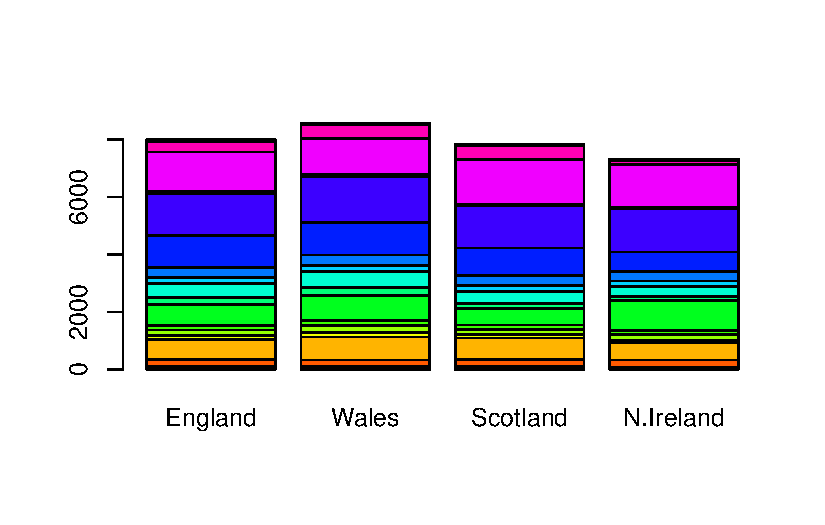
\includegraphics{Lab-7_files/figure-pdf/unnamed-chunk-19-1.pdf}

}

\end{figure}

\begin{Shaded}
\begin{Highlighting}[]
\CommentTok{\# Q3: We set beside=FALSE to change the barplot into a stacked format instead of the bars being side by side.}
\end{Highlighting}
\end{Shaded}

\begin{Shaded}
\begin{Highlighting}[]
\CommentTok{\# Generating pairwise plots. }
\FunctionTok{pairs}\NormalTok{(x, }\AttributeTok{col=}\FunctionTok{rainbow}\NormalTok{(}\DecValTok{10}\NormalTok{), }\AttributeTok{pch=}\DecValTok{16}\NormalTok{)}
\end{Highlighting}
\end{Shaded}

\begin{figure}[H]

{\centering 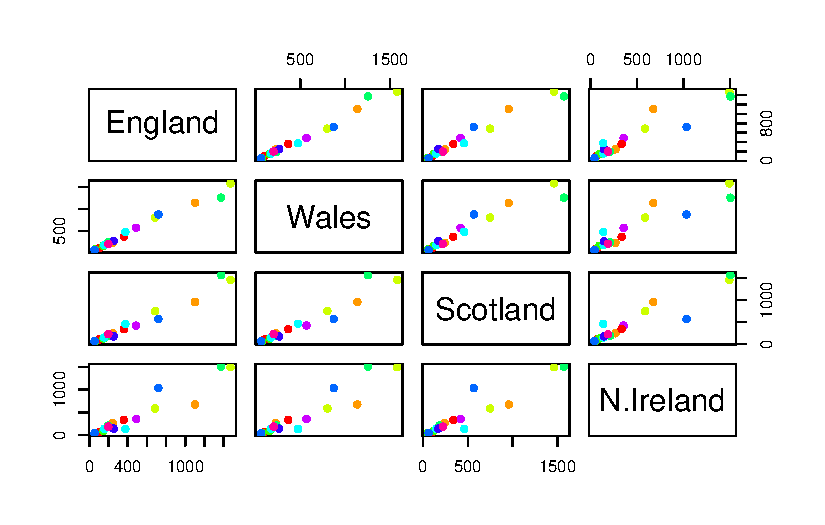
\includegraphics{Lab-7_files/figure-pdf/unnamed-chunk-20-1.pdf}

}

\end{figure}

\begin{Shaded}
\begin{Highlighting}[]
\CommentTok{\# Q5: If a point lines on the diagonal, then that means that the country on the y{-}axis and the country on the x{-}axis have the same amount of that product. }
\end{Highlighting}
\end{Shaded}

\begin{quote}
Q5: If a datapoint is on the diagonal, then the countries have the same
amount of that product. If a datapoint is above the diagonal then the
country on the y-axis has a higher amount of that product. If a
datapoint is below the diagonal line (i.e.~further to the right) then
the country on the x-axis has more of that product.
\end{quote}

\begin{quote}
Q6: N. Ireland has more of the blue datapoint than other countries,
since that datapoint is further to the right on the graph (below
diagonal) when N. Ireland is plotted on the x-axis, and higher up on the
graph (above diagonal) when N. Ireland is plotted on the y-axis.
\end{quote}

The main PCA function in base R is called \texttt{prcomp()} it expects
the transpose of our data.

\begin{Shaded}
\begin{Highlighting}[]
\NormalTok{pca }\OtherTok{\textless{}{-}} \FunctionTok{prcomp}\NormalTok{( }\FunctionTok{t}\NormalTok{(x) )}
\FunctionTok{summary}\NormalTok{(pca)}
\end{Highlighting}
\end{Shaded}

\begin{verbatim}
Importance of components:
                            PC1      PC2      PC3       PC4
Standard deviation     324.1502 212.7478 73.87622 4.189e-14
Proportion of Variance   0.6744   0.2905  0.03503 0.000e+00
Cumulative Proportion    0.6744   0.9650  1.00000 1.000e+00
\end{verbatim}

\begin{Shaded}
\begin{Highlighting}[]
\FunctionTok{attributes}\NormalTok{(pca)}
\end{Highlighting}
\end{Shaded}

\begin{verbatim}
$names
[1] "sdev"     "rotation" "center"   "scale"    "x"       

$class
[1] "prcomp"
\end{verbatim}

\begin{Shaded}
\begin{Highlighting}[]
\CommentTok{\# Q7: Competing the pca plot code.}
\FunctionTok{plot}\NormalTok{(pca}\SpecialCharTok{$}\NormalTok{x[,}\DecValTok{1}\NormalTok{], pca}\SpecialCharTok{$}\NormalTok{x[,}\DecValTok{2}\NormalTok{], }
     \AttributeTok{xlab=}\StringTok{"PC1"}\NormalTok{, }\AttributeTok{ylab=}\StringTok{"PC2"}\NormalTok{, }
     \AttributeTok{col =} \StringTok{\textquotesingle{}transparent\textquotesingle{}}\NormalTok{, }
     \AttributeTok{pch =} \DecValTok{16}\NormalTok{, }
     \AttributeTok{xlim=}\FunctionTok{c}\NormalTok{(}\SpecialCharTok{{-}}\DecValTok{270}\NormalTok{,}\DecValTok{500}\NormalTok{))}

\CommentTok{\# Q8: Customizing the plot by adding color.}
\FunctionTok{text}\NormalTok{(pca}\SpecialCharTok{$}\NormalTok{x[,}\DecValTok{1}\NormalTok{], pca}\SpecialCharTok{$}\NormalTok{x[,}\DecValTok{2}\NormalTok{], }
     \FunctionTok{colnames}\NormalTok{(x), }
     \AttributeTok{col =} \FunctionTok{c}\NormalTok{(}\StringTok{"orange"}\NormalTok{, }\StringTok{"red"}\NormalTok{, }\StringTok{"blue"}\NormalTok{, }\StringTok{"darkgreen"}\NormalTok{))}
\end{Highlighting}
\end{Shaded}

\begin{figure}[H]

{\centering 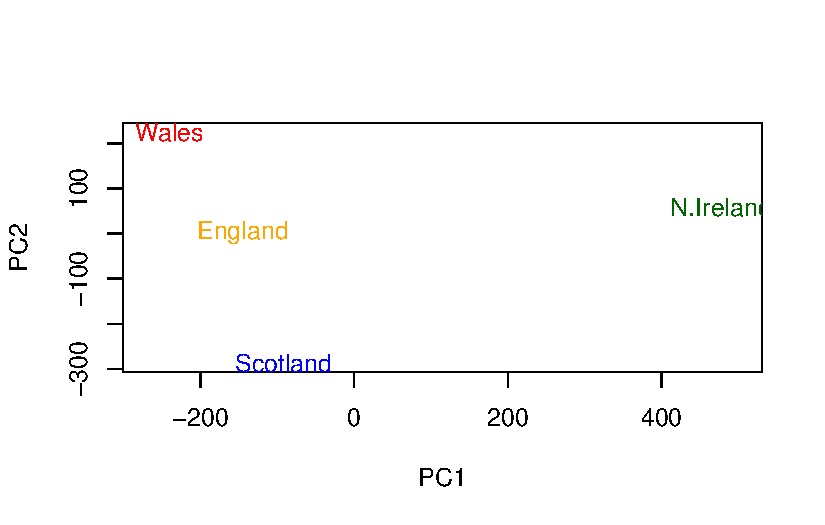
\includegraphics{Lab-7_files/figure-pdf/unnamed-chunk-23-1.pdf}

}

\end{figure}



\end{document}
